\documentclass[12pt]{report}\usepackage[]{graphicx}\usepackage[dvipsnames]{xcolor}
% maxwidth is the original width if it is less than linewidth
% otherwise use linewidth (to make sure the graphics do not exceed the margin)
\makeatletter
\def\maxwidth{ %
  \ifdim\Gin@nat@width>\linewidth
    \linewidth
  \else
    \Gin@nat@width
  \fi
}
\makeatother

\definecolor{fgcolor}{rgb}{0.345, 0.345, 0.345}
\newcommand{\hlnum}[1]{\textcolor[rgb]{0.686,0.059,0.569}{#1}}%
\newcommand{\hlstr}[1]{\textcolor[rgb]{0.192,0.494,0.8}{#1}}%
\newcommand{\hlcom}[1]{\textcolor[rgb]{0.678,0.584,0.686}{\textit{#1}}}%
\newcommand{\hlopt}[1]{\textcolor[rgb]{0,0,0}{#1}}%
\newcommand{\hlstd}[1]{\textcolor[rgb]{0.345,0.345,0.345}{#1}}%
\newcommand{\hlkwa}[1]{\textcolor[rgb]{0.161,0.373,0.58}{\textbf{#1}}}%
\newcommand{\hlkwb}[1]{\textcolor[rgb]{0.69,0.353,0.396}{#1}}%
\newcommand{\hlkwc}[1]{\textcolor[rgb]{0.333,0.667,0.333}{#1}}%
\newcommand{\hlkwd}[1]{\textcolor[rgb]{0.737,0.353,0.396}{\textbf{#1}}}%
\let\hlipl\hlkwb

\usepackage{framed}
\makeatletter
\newenvironment{kframe}{%
 \def\at@end@of@kframe{}%
 \ifinner\ifhmode%
  \def\at@end@of@kframe{\end{minipage}}%
  \begin{minipage}{\columnwidth}%
 \fi\fi%
 \def\FrameCommand##1{\hskip\@totalleftmargin \hskip-\fboxsep
 \colorbox{shadecolor}{##1}\hskip-\fboxsep
     % There is no \\@totalrightmargin, so:
     \hskip-\linewidth \hskip-\@totalleftmargin \hskip\columnwidth}%
 \MakeFramed {\advance\hsize-\width
   \@totalleftmargin\z@ \linewidth\hsize
   \@setminipage}}%
 {\par\unskip\endMakeFramed%
 \at@end@of@kframe}
\makeatother

\definecolor{shadecolor}{rgb}{.97, .97, .97}
\definecolor{messagecolor}{rgb}{0, 0, 0}
\definecolor{warningcolor}{rgb}{1, 0, 1}
\definecolor{errorcolor}{rgb}{1, 0, 0}
\newenvironment{knitrout}{}{} % an empty environment to be redefined in TeX

\usepackage{alltt}

\usepackage[spanish]{babel}
\usepackage[margin=2.54cm]{geometry}
\usepackage[dvipsnames]{xcolor}
\usepackage{array, amssymb, amsthm, enumitem, fancyhdr, float, graphicx, hyperref, hologo, mathtools, tikz, tikz-cd}
\usepackage[spanish, noabbrev]{cleveref}

\pagestyle{fancy}
\lhead{\footnotesize \leftmark}
\rhead{\footnotesize \rightmark}

\title{
	\huge
	\noindent\textbf{Fundamentos de la Ciencia de Datos}\\
	
	{\Large \textit{Práctica 1}}
	\vspace{1cm}
	
	\huge
	Grado en Ingeniería Informática\\
	Universidad de Alcalá\\
	
	\vspace{1cm}
	
	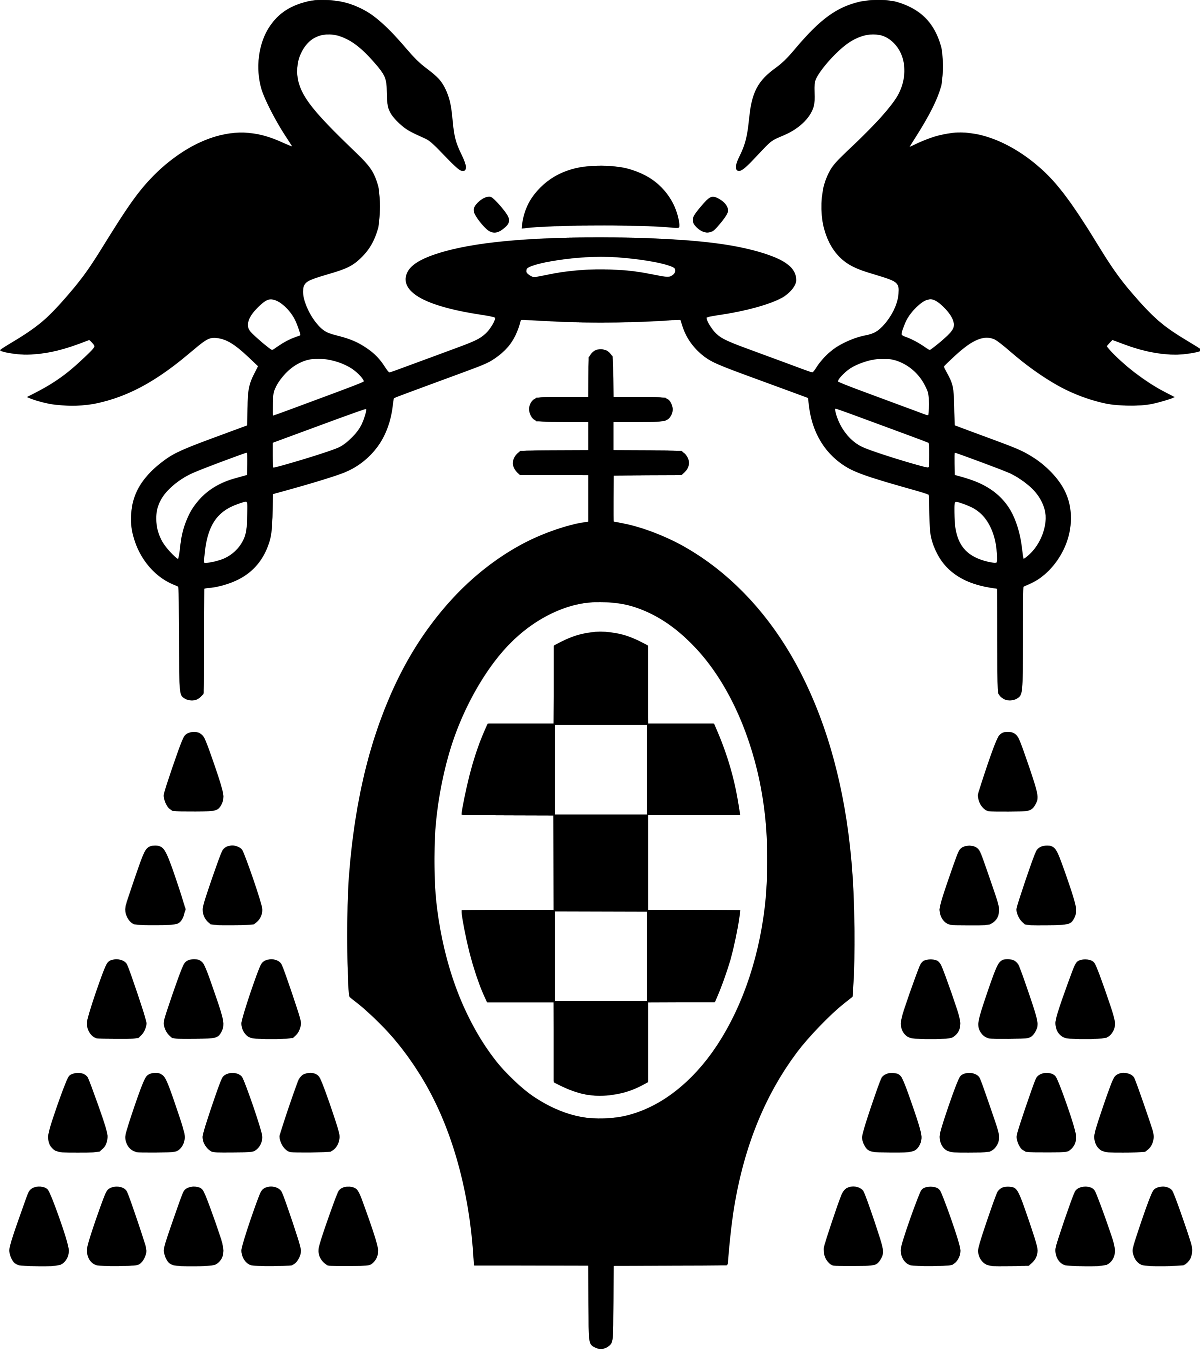
\includegraphics[scale=0.075]{img/logo}
}

\author{
	Pablo García García\\
	Abel López Martínez\\
	Álvaro Jesús Martínez Parra\\
	Raúl Moratilla Núñez
}

\date{
	\large{14 de noviembre de 2023}
}

\hypersetup{
	pdftitle={Práctica 1}, 
	pdfauthor={Pablo García García, Abel López Martínez, Álvaro Jesús Martínez Parra, Raúl Moratilla Núñez}, 
	pdfsubject={Fundamentos de la Ciencia de Datos}, 
	pdfcenterwindow, 
	pdfnewwindow=true, 
	pdfkeywords={Entrega de la PL1 de laboratorio correspondiente al Curso 2023-2024}, 
	bookmarksopen=true 
}
\IfFileExists{upquote.sty}{\usepackage{upquote}}{}
\begin{document}
	
	\renewcommand{\chaptername}{Parte}
	\maketitle \thispagestyle{empty}
	
	\newpage
	
	\tableofcontents
	\listoffigures
	
	\chapter*{Introducción}\addcontentsline{toc}{chapter}{Introducción}\pagestyle{plain}
	
		\section*{El lenguaje R}\addcontentsline{toc}{section}{El lenguaje R}
		
			El lenguaje R, es un software de uso gratuito comúnmente usado en tareas relacionadas con la estadística, como el análisis o visualización de datos; o en general la propia Ciencia de Datos. Para ello cuenta con una gran cantidad de paquetes y herramientas que facilitan el trabajo.  
			
			\begin{figure}[H]
				\centering
				
\includegraphics[scale = 0.15]{img/Rlogo}
				\caption{Logo del lenguaje R}
				\label{fig:logo_R}
			\end{figure}
		
			El CRAN (Comprehensive R Archive Network, \url{https://cran.r-project.org/}) es un repositorio de recursos en línea que se utiliza para facilitar la distribución, el intercambio y el acceso a una amplia gama de software y paquetes relacionados con el lenguaje de programación R. La página web de CRAN sirve como el portal central para acceder a estos recursos y ofrece una variedad de apartados y enlaces útiles para los usuarios de R. A continuación, proporcionamos una descripción de los distintos enlaces a los que se puede acceder desde la página principal del CRAN: 
			
			\begin{itemize}
				\item Mirrors: Esta sección permite a los usuarios seleccionar un espejo (mirror) cercano para descargar paquetes y recursos. Los espejos son servidores que almacenan copias de los paquetes y datos de CRAN, lo que ayuda a mejorar la velocidad de descarga y la disponibilidad de los recursos.
				
				\item What's new?: En esta sección, los usuarios pueden encontrar información sobre las últimas actualizaciones y novedades en el mundo de R y los paquetes disponibles en CRAN. Esto es útil para estar al tanto de las últimas características y mejoras.
				
				\item Search: El enlace ``Search'' permite a los usuarios buscar paquetes y recursos específicos en el repositorio de CRAN. Además, se puede utilizar la función de búsqueda avanzada del motor de búsqueda de Google.
				
				\item CRAN Team: Aquí se puede encontrar información sobre las personas y equipos que trabajan en el mantenimiento y desarrollo de CRAN. Es útil para conocer a las personas detrás de esta valiosa fuente de recursos.
				
				\item About R: Esta sección proporciona información sobre el lenguaje de programación R en general. Incluye enlaces a la página de inicio de R y a ``The R Journal'', una publicación académica relacionada con R.
				
				\item Software: Esta sección ofrece acceso a diversas fuentes y binarios relacionados con R, lo que permite a los usuarios descargar e instalar R en su sistema. También proporciona acceso a paquetes, Task Views y otros recursos.
				
				\item Documentation: Aquí los usuarios pueden encontrar documentación esencial relacionada con R. Esto incluye manuales, preguntas frecuentes (FAQs) y contribuciones de la comunidad para ayudar a los usuarios a comprender y utilizar R de manera efectiva.
			\end{itemize}
		
			%EXPLICAR INSTALACION PAQUETES
		
		\section*{El lenguaje \LaTeX}\addcontentsline{toc}{section}{El lenguaje \LaTeX}

			Para la realización de esta práctica, se empleará el concepto de \textbf{programación literaria}, que consiste en crear un documento en el que se combine texto con código, de manera que este se pueda explicar y entender de una manera mucho más sencilla. Una forma de realizar esto con código R, es el uso del lenguaje \LaTeX{}, que es un sistema de composición de documentos enfocado al ámbito científico. Es algo similar a un lenguaje de marcas con el que poder definir la estructura de un documento, pero cuenta con la particularidad de que es un lenguaje Turing--completo, por lo que cualquier algoritmo puede ser implementado dando una mayor flexibilidad, aunque no sea su objetivo principal. Veremos ahora los pasos seguidos para su instalación. Para poder trabajar, lo mínimo que necesitaremos es un compilador de \LaTeX{}, en este caso se ha optado por la distribución \hologo{MiKTeX} que lo incluye, ya que estamos trabajando en Windows. Además, para una mayor comodidad trabajando con el código, se ha optado por el IDE \TeX{}studio, uno de los más conocidos en la comunidad. \\
			
			Una vez hemos tratado ambos lenguajes, necesitamos entender con qué tipos de extensiones se suelen trabajar para ver el proceso de integración con R (sin entrar en profundidad). Estas dependen de cómo queremos almacenar nuestro documento, o cómo están almacenadas dependencias de estos, como por ejemplo, imágenes. Esta tarea se realiza usando un compilador u otro. \\
			
			Para ello nos fijaremos en la \Cref{fig:extensiones}. Por ahora nos quedaremos con las extensiones que trabajaremos más a menudo, que serán \texttt{.Rnw}, \texttt{.tex}, y \texttt{.pdf}. La primera de ellas representan los archivos que tienen código \LaTeX{} y R ``mezclado'', la segunda aquellos que contienen código \LaTeX{} puro, y la última nuestro documento final. \\
			
			\begin{figure}
				\centering
				\begin{tikzcd}
					& \texttt{.Rnw} \arrow[d] & \\
					& \texttt{.tex} \arrow[ld] \arrow[rd] \arrow[dd] & \\
					\texttt{.dvi} \arrow[rr] \arrow[rd] & & \texttt{.ps} \arrow[ld] \\
					& \texttt{.pdf} &               
				\end{tikzcd}
				\caption{Esquema de extensiones en \LaTeX}
				\label{fig:extensiones}
			\end{figure}
			
			Existen dos herramientas que nos permiten trabajar con archivos \texttt{.Rnw}, estas son Sweave y Knitr. A pesar de que en la asignatura ha sido propuesta la primera de ellas, optaremos por la segunda, pues existieron diversos errores al compilar archivos con esta, y al ser más antigua, los documentos finales tenían menos calidad. Knitr nos ofrece mayor calidad y un mejor formato en el código fuente R mostrado. Para instalarla basta con escribir \texttt{install.packages('knitr')} en una consola de R. Sweave viene ya por defecto con \texttt{utils}. \\
			
			Por último, se explicará cómo hemos agilizado el proceso de trabajo con Knitr y \TeX{}Studio. Lo primero será hacer que R cargue por defecto Knitr, para ello modificaremos el archivo \texttt{Rprofile} en \texttt{libray/base/R} dentro de la carpeta de instalación de R, añadiendo \texttt{knitr} al resto de paquetes que carga por defecto. Una vez hecho esto, iremos a la configuración de \TeX{}Studio, y aquí a \textit{Compilar}. En la zona \textit{Órdenes de usuario}, crearemos una nueva tal y como se ve en la \Cref{fig:orden}, de manera que le digamos dónde están los binarios de R, para que pueda crear un fichero \texttt{.tex}, y posteriormente invocar a nuestro compilador, para obtener nuestro documento en \texttt{.pdf}. \TeX{}Studio se encargará de reemplazar el símbolo \% por el nombre del archivo que le ordenamos compilar. 
			
			\begin{figure}[H]
				\centering
				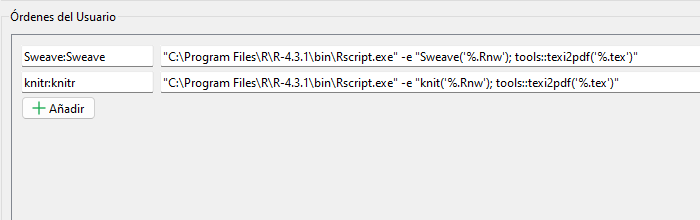
\includegraphics[scale = 0.7]{img/o_usuario}
				\caption{Creación de orden de usuario}
				\label{fig:orden}
			\end{figure}
			
			Ahora basta modificar el botón verde del IDE para que en vez de invocar al compilador \hologo{pdfLaTeX}, lleve a cabo la instrucción que le hemos dado. Para ello volveremos al menú de compilación en el que nos ubicábamos previamente, y observaremos la sección de \textit{Meta-Órdenes}. Modificaremos el valor del campo \textit{Compilador por defecto}, escribiendo \texttt{txs:///knitr} para que se ejecute la orden que previamente hemos creado, o podemos hacerlo de manera gráfica como se observa en la \Cref{fig:comp}. Ahora bastará pulsar el botón verde o F5 para ver a nuestra izquierda el código de nuestro documento, y a la derecha actualizado, el documento PDF final. 
			
			\begin{figure}[H]
				\centering
				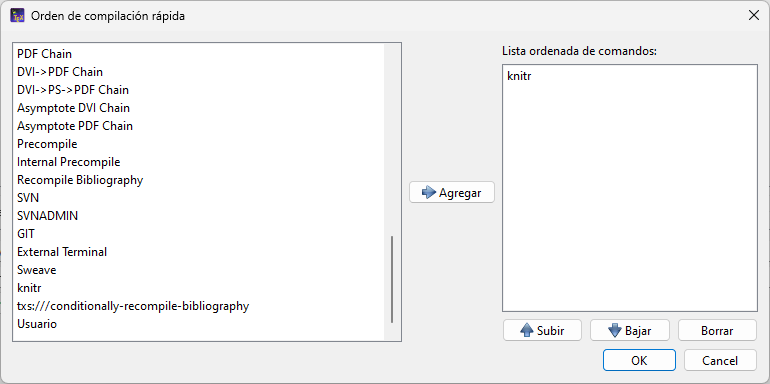
\includegraphics[scale = 0.7]{img/compilacion}
				\caption{Modificación de compilación}
				\label{fig:comp}
			\end{figure}
			
			Por último, para llevar un mejor control de versiones del proyecto, y de coordinación entre los miembros del grupo, se usará un repositorio de GitHub. Añadiremos un archivo \texttt{.gitignore} para no cargar en el repositorio los archivos temporales generados durante la compilación. Otra alternativa que se podría haber usado, es usar Overleaf (aquí usaríamos la extensión \texttt{.Rtex} en vez de \texttt{.Rnw}), ya que no sería necesaria la instalación de ningún software, y también trabaja con Knitr. Sin embargo, la integración de GitHub en Overleaf es de pago, por lo que optamos por usar la configuración explicada hasta el momento, para poder tener un mejor control de versiones sin coste alguno. \\
			
			Por último, mencionar que al igual que R posee su repositorio de paquetes (que ya hemos visto que incluye más cosas) llamado CRAN, \LaTeX{} que en realidad es ``un subconjunto'' del lenguaje \TeX{}, también tiene su propio portal llamado CTAN o Comprehensive \TeX{} Archive Network (\url{https://www.ctan.org/}) de donde se descargan los paquetes y otros materiales para el lenguaje. 
			
			\begin{figure}[H]
				\centering
				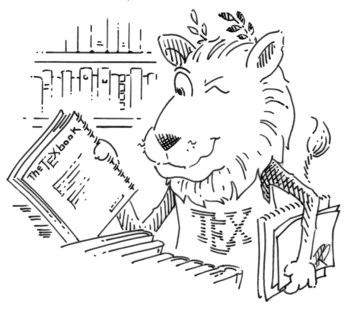
\includegraphics[scale = 0.5]{img/ctan_lion}
				\caption{Mascota de \TeX{} y el CTAN}
				\label{fig:leon}
			\end{figure}
			
	\chapter{Ejercicios guiados}\pagestyle{fancy}
	
		En esta primera parte de esta práctica, repetirán los ejercicios explicados y realizados por el profesor en las clases de laboratorio, utilizando los mismos procedimientos vistos plasmándolos en este documento. 
	
		\section{Descripción de los datos}
		
			``\textit{El primer conjunto de datos, que se empleará para realizar el análisis de descripción de datos, estará formado por datos de una característica cualitativa, nombre, y otra cuantitativa, radio, de los satélites menores de Urano, es decir, aquellos que tienen un radio menor de 50 Km, dichos datos, los primeros cualitativos nominales, y los segundos cuantitativos continuos, son: (Nombre, radio en Km): Cordelia, 13; Ofelia, 16; Bianca, 22; Crésida, 33; Desdémona, 29; Julieta, 42; Rosalinda, 27; Belinda, 34; Luna-1986U10, 20; Calíbano, 30; Luna-999U1, 20; Luna 1999U2, 15.}''\\
			
			Para comenzar con la resolución de este ejercicio, deberemos escribir los datos en un fichero \texttt{.txt}, cumpliendo las siguientes normas: 
			
			\begin{itemize}
				\item Existirá una tabulación entre dato y dato. 
				\item La primera columna numera las filas, y en la primera fila se introduce un espacio y el nombre de las variables. 
				\item Se introducirá un salto de línea en la última fila
				\item Para los números decimales se utilizarán puntos. 
				\item Al escribir nombres, no se deberán introducir espacios. 
			\end{itemize}
			
			Obedeciendo a estas normas, copiamos los datos en un fichero llamado \texttt{satelites.txt}, y lo cargamos en R de la siguiente manera: 
			
\begin{knitrout}
\definecolor{shadecolor}{rgb}{0.969, 0.969, 0.969}\color{fgcolor}\begin{kframe}
\begin{alltt}
\hlstd{s} \hlkwb{<-} \hlkwd{read.table}\hlstd{(}\hlstr{"data/satelites.txt"}\hlstd{)}
\hlkwd{print}\hlstd{(s)}
\end{alltt}
\begin{verbatim}
##          nombre radio
## 1      Cordelia    13
## 2        Ofelia    16
## 3        Bianca    22
## 4       Crésida    33
## 5     Desdémona    29
## 6       Julieta    42
## 7     Rosalinda    27
## 8       Belinda    34
## 9  Luna-1986U10    20
## 10     Calíbano    30
## 11   Luna-999U1    20
## 12  Luna-1999U2    15
\end{verbatim}
\end{kframe}
\end{knitrout}
			
			Ahora en la variable \texttt{s} tenemos un dataframe con los datos de nuestros satélites. En los dataframes se accede por \texttt{[fila, columna]}, y también podemos consultar las dimensiones con la función \texttt{dim}. Sería de esperar que nos dijera que tiene 12 filas (los 12 datos), y 2 columnas (\texttt{nombre} y \texttt{radio}). 
			
\begin{knitrout}
\definecolor{shadecolor}{rgb}{0.969, 0.969, 0.969}\color{fgcolor}\begin{kframe}
\begin{alltt}
\hlkwd{dim}\hlstd{(s)}
\end{alltt}
\begin{verbatim}
## [1] 12  2
\end{verbatim}
\end{kframe}
\end{knitrout}
			
			También podemos ordenar el dataframe, en función de una de las magnitudes (columnas), usando la función \texttt{order} aplicando recursivamente el concepto de acceder por filas y columnas. Veamos un ejemplo, si en \texttt{s} teníamos guardado nuestro dataframe, y queremos ordenar por \texttt{radio}, la manera de hacerlo sería la siguiente: 
			
\begin{knitrout}
\definecolor{shadecolor}{rgb}{0.969, 0.969, 0.969}\color{fgcolor}\begin{kframe}
\begin{alltt}
\hlstd{s_ordered} \hlkwb{<-} \hlstd{s[}\hlkwd{order}\hlstd{(s}\hlopt{$}\hlstd{radio), ]}
\hlkwd{print}\hlstd{(s_ordered)}
\end{alltt}
\begin{verbatim}
##          nombre radio
## 1      Cordelia    13
## 12  Luna-1999U2    15
## 2        Ofelia    16
## 9  Luna-1986U10    20
## 11   Luna-999U1    20
## 3        Bianca    22
## 7     Rosalinda    27
## 5     Desdémona    29
## 10     Calíbano    30
## 4       Crésida    33
## 8       Belinda    34
## 6       Julieta    42
\end{verbatim}
\end{kframe}
\end{knitrout}
			
			Podemos introducir nuevos criterios a la ordenación, como por ejemplo, hacerlo en orden descendente. Para esto usaremos la función \texttt{rev}. 
			
\begin{knitrout}
\definecolor{shadecolor}{rgb}{0.969, 0.969, 0.969}\color{fgcolor}\begin{kframe}
\begin{alltt}
\hlstd{s_ordered_rev} \hlkwb{<-} \hlstd{s[}\hlkwd{rev}\hlstd{(}\hlkwd{order}\hlstd{(s}\hlopt{$}\hlstd{radio)), ]}
\hlkwd{print}\hlstd{(s_ordered_rev)}
\end{alltt}
\begin{verbatim}
##          nombre radio
## 6       Julieta    42
## 8       Belinda    34
## 4       Crésida    33
## 10     Calíbano    30
## 5     Desdémona    29
## 7     Rosalinda    27
## 3        Bianca    22
## 11   Luna-999U1    20
## 9  Luna-1986U10    20
## 2        Ofelia    16
## 12  Luna-1999U2    15
## 1      Cordelia    13
\end{verbatim}
\end{kframe}
\end{knitrout}
			
			También suele ser útil conocer cuántos elementos tiene una columna. Podemos averiguarlo con la función \texttt{length}, veamos un ejemplo. 
			
\begin{knitrout}
\definecolor{shadecolor}{rgb}{0.969, 0.969, 0.969}\color{fgcolor}\begin{kframe}
\begin{alltt}
\hlkwd{length}\hlstd{(s}\hlopt{$}\hlstd{radio)}
\end{alltt}
\begin{verbatim}
## [1] 12
\end{verbatim}
\end{kframe}
\end{knitrout}
			
			Otro valor que nos podemos plantear calcular es el rango. Para ello podemos usar las funciones \texttt{max} y \texttt{min}. Debemos tener cuidado con la función \texttt{range} y no confundirnos, pues nos dará los valores máximo y mínimo. 
			
\begin{knitrout}
\definecolor{shadecolor}{rgb}{0.969, 0.969, 0.969}\color{fgcolor}\begin{kframe}
\begin{alltt}
\hlstd{r} \hlkwb{<-} \hlkwd{max}\hlstd{(s}\hlopt{$}\hlstd{radio)} \hlopt{-} \hlkwd{min}\hlstd{(s}\hlopt{$}\hlstd{radio)}
\hlkwd{print}\hlstd{(r)}
\end{alltt}
\begin{verbatim}
## [1] 29
\end{verbatim}
\begin{alltt}
\hlkwd{range}\hlstd{(s}\hlopt{$}\hlstd{radio)}
\end{alltt}
\begin{verbatim}
## [1] 13 42
\end{verbatim}
\end{kframe}
\end{knitrout}
			
			Para una mejor lectura, podemos cambiar la forma de obtener la columna de los radios: 
			
\begin{knitrout}
\definecolor{shadecolor}{rgb}{0.969, 0.969, 0.969}\color{fgcolor}\begin{kframe}
\begin{alltt}
\hlstd{radio} \hlkwb{<-} \hlstd{s}\hlopt{$}\hlstd{radio}
\end{alltt}
\end{kframe}
\end{knitrout}
			
			La idea de calcular la diferencia de el máximo y el mínimo a mano parece funcionar, sin embargo, para futuros casos sería más ágil tener codificada una función como la siguiente. 
			
\begin{knitrout}
\definecolor{shadecolor}{rgb}{0.969, 0.969, 0.969}\color{fgcolor}\begin{kframe}
\begin{alltt}
\hlstd{rango} \hlkwb{<-} \hlkwa{function}\hlstd{(}\hlkwc{radio}\hlstd{)\{}\hlkwd{max}\hlstd{(radio)} \hlopt{-} \hlkwd{min}\hlstd{(radio)\}}
\hlkwd{rango}\hlstd{(radio)}
\end{alltt}
\begin{verbatim}
## [1] 29
\end{verbatim}
\end{kframe}
\end{knitrout}
			
			Sin embargo, al salir de R, la definición de la función se pierde, por lo que deberemos guardarla en un fichero, y posteriormente cargarlo en futuras ejecuciones. Lo haremos de la siguiente manera: 
			
\begin{knitrout}
\definecolor{shadecolor}{rgb}{0.969, 0.969, 0.969}\color{fgcolor}\begin{kframe}
\begin{alltt}
\hlkwd{dump}\hlstd{(}\hlstr{"rango"}\hlstd{,} \hlkwc{file} \hlstd{=} \hlstr{"fn/rango.R"}\hlstd{)}
\hlkwd{source}\hlstd{(}\hlstr{"fn/rango.R"}\hlstd{)}
\end{alltt}
\end{kframe}
\end{knitrout}
			
			Volviendo al estudio de nuestros datos, veamos cómo calcular las diferentes frecuencias. Como en R no existe una función para las frecuencias relativas, se definirá y guardará una propia. 
			
\begin{knitrout}
\definecolor{shadecolor}{rgb}{0.969, 0.969, 0.969}\color{fgcolor}\begin{kframe}
\begin{alltt}
\hlstd{fabs_radio} \hlkwb{<-} \hlkwd{table}\hlstd{(radio)}
\hlstd{fabsacum_radio} \hlkwb{<-} \hlkwd{cumsum}\hlstd{(fabs_radio)}
\hlstd{frecrel} \hlkwb{<-} \hlkwa{function}\hlstd{(}\hlkwc{r}\hlstd{)\{}\hlkwd{table}\hlstd{(r)}\hlopt{/}\hlkwd{length}\hlstd{(r)\}}
\hlkwd{dump}\hlstd{(}\hlstr{"frecrel"}\hlstd{,} \hlkwc{file} \hlstd{=} \hlstr{"fn/frecrel.R"}\hlstd{)}

\hlkwd{print}\hlstd{(fabs_radio)}
\end{alltt}
\begin{verbatim}
## radio
## 13 15 16 20 22 27 29 30 33 34 42 
##  1  1  1  2  1  1  1  1  1  1  1
\end{verbatim}
\begin{alltt}
\hlkwd{print}\hlstd{(fabsacum_radio)}
\end{alltt}
\begin{verbatim}
## 13 15 16 20 22 27 29 30 33 34 42 
##  1  2  3  5  6  7  8  9 10 11 12
\end{verbatim}
\begin{alltt}
\hlkwd{print}\hlstd{(}\hlkwd{frecrel}\hlstd{(radio))}
\end{alltt}
\begin{verbatim}
## r
##         13         15         16         20         22         27         29 
## 0.08333333 0.08333333 0.08333333 0.16666667 0.08333333 0.08333333 0.08333333 
##         30         33         34         42 
## 0.08333333 0.08333333 0.08333333 0.08333333
\end{verbatim}
\end{kframe}
\end{knitrout}
			
			Otro valor que podemos calcular es la media aritmética de los datos, para ello se cuenta con la función \texttt{mean}. 
			
\begin{knitrout}
\definecolor{shadecolor}{rgb}{0.969, 0.969, 0.969}\color{fgcolor}\begin{kframe}
\begin{alltt}
\hlstd{mr} \hlkwb{<-} \hlkwd{mean}\hlstd{(radio)}
\hlkwd{print}\hlstd{(mr)}
\end{alltt}
\begin{verbatim}
## [1] 25.08333
\end{verbatim}
\end{kframe}
\end{knitrout}
			
			Ahora calcularemos la desviación típica, para ello se cuenta con la función \texttt{sd}. 
			
\begin{knitrout}
\definecolor{shadecolor}{rgb}{0.969, 0.969, 0.969}\color{fgcolor}\begin{kframe}
\begin{alltt}
\hlstd{sdr} \hlkwb{<-} \hlkwd{sd}\hlstd{(radio)}
\hlkwd{print}\hlstd{(sdr)}
\end{alltt}
\begin{verbatim}
## [1] 8.857029
\end{verbatim}
\end{kframe}
\end{knitrout}
			
			Sin embargo, el resultado obtenido no es el esperado. Esto se debe a que esta función realiza el siguiente cálculo
			$$
			\sigma = \sqrt{\frac{\displaystyle\sum_{i=0}^n (x_i-\bar{x})^2}{n-1}}
			$$
			que es más utilizado en inferencia estadística, porque hace que se parezca más a una campana de Gauss (menos sesgo), mientras que la fórmula vista en clase utiliza un factor de $n$ en vez de $n-1$ en el denominador (dentro de la raíz). Para ello, el profesor lo corrigió de la siguiente manera: 
			
\begin{knitrout}
\definecolor{shadecolor}{rgb}{0.969, 0.969, 0.969}\color{fgcolor}\begin{kframe}
\begin{alltt}
\hlstd{sdr2} \hlkwb{<-} \hlkwd{sqrt}\hlstd{((sdr}\hlopt{^}\hlnum{2}\hlstd{)}\hlopt{*}\hlstd{(}\hlkwd{length}\hlstd{(radio)}\hlopt{-}\hlnum{1}\hlstd{)}\hlopt{/}\hlkwd{length}\hlstd{(radio))}
\hlkwd{print}\hlstd{(sdr2)}
\end{alltt}
\begin{verbatim}
## [1] 8.47996
\end{verbatim}
\end{kframe}
\end{knitrout}
			
			En realidad lo que se está realizando es el siguiente ``ajuste'': 
			$$
			\sigma' = \sqrt{\sigma^2\cdot\frac{n-1}{n}}
			$$
			
			Una vez hemos visto cómo se calcula la desviación típica, podremos ver cómo calcular la varianza. Como sabemos que es el cuadrado de la desviación típica, bastaría con elevar al cuadrado si no fuera por el ``fallo'' de $n-1$ visto previamente. En este caso, el profesor lo arregló para el caso particular de la siguiente manera: 
			
\begin{knitrout}
\definecolor{shadecolor}{rgb}{0.969, 0.969, 0.969}\color{fgcolor}\begin{kframe}
\begin{alltt}
\hlstd{varr} \hlkwb{<-} \hlkwd{var}\hlstd{(radio)}
\hlstd{varr} \hlkwb{<-} \hlnum{11}\hlopt{/}\hlnum{12} \hlopt{*} \hlstd{varr}
\hlkwd{print}\hlstd{(varr)}
\end{alltt}
\begin{verbatim}
## [1] 71.90972
\end{verbatim}
\end{kframe}
\end{knitrout}
			
			Otro de los valores que se ha enseñado cómo calcular, es la mediana. Para este caso existe la función \texttt{median}. 
			
\begin{knitrout}
\definecolor{shadecolor}{rgb}{0.969, 0.969, 0.969}\color{fgcolor}\begin{kframe}
\begin{alltt}
\hlstd{medianr} \hlkwb{<-} \hlkwd{median}\hlstd{(radio)}
\hlkwd{print}\hlstd{(medianr)}
\end{alltt}
\begin{verbatim}
## [1] 24.5
\end{verbatim}
\end{kframe}
\end{knitrout}
			
			En último lugar, el profesor enseñó cómo calcular cuantiles, y para ello mostró la función \texttt{quantile}, pero se mencionó que se obtienen resultados diferentes a los esperados debido a la forma que tiene de calcularlos, y se deberá programar. Aquí se muestra un ejemplo de cómo se calcularía el primer cuartil. 
			
\begin{knitrout}
\definecolor{shadecolor}{rgb}{0.969, 0.969, 0.969}\color{fgcolor}\begin{kframe}
\begin{alltt}
\hlstd{cuar1} \hlkwb{<-} \hlkwd{quantile}\hlstd{(radio,} \hlnum{0.25}\hlstd{)}
\hlkwd{print}\hlstd{(cuar1)}
\end{alltt}
\begin{verbatim}
## 25% 
##  19
\end{verbatim}
\end{kframe}
\end{knitrout}
			
			Como añadido, el profesor explicó cómo abrir un ejemplo de Sweave, cómo pasarlo a un fichero que \LaTeX{} pudiese leer, y cómo compilarlo a PDF. Las instrucciones son las que se verán a continuación, aunque como ya se explicó en la introducción, usaremos otra forma de trabajar con estos archivos a lo largo de la práctica. 
			
			\begin{verbatim}
				rnwfile<-system.file("Sweave", "example-1.Rnw", package="utils")
				Sweave(rnwfile)
				tools::texi2pdf("example-1.tex")
			\end{verbatim}
		
		\section{Asociación}
		
			``\textit{El segundo conjunto de datos, que se empleará para realizar el análisis de asociación, estará formado por las siguientes 6 cestas de la compra: \{Pan, Agua, Leche, Naranjas\}, \{Pan, Agua, Café, Leche\}, \{Pan, Agua, Leche\}, \{Pan, Café, Leche\}, \{Pan, Agua\}, \{Leche\}.}''
		
		\section{Detección de datos anómalos}
		
			\subsection{Primer ejercicio}
			
				``\textit{El tercer conjunto de datos, que se empleará para realizar el análisis de detección de datos anómalos utilizando técnicas con base estadística, estará formado por los siguientes 7 valores de resistencia y densidad para diferentes tipos de hormigón \{Resistencia, Densidad\}: \{3, 2; 3.5, 12; 4.7, 4.1; 5.2, 4.9; 7.1, 6.1; 6.2, 5.2; 14, 5.3\}. Aplicar las medidas de ordenación a la resistencia y las de dispersión a la densidad.}''\\
				
				Lo primero explicado por el profesor fue la preparación de los datos proporcionados para que \texttt{arules} fuese capaz de tratar con ellos. Para ello se introduce una matriz de ceros y unos mediante el paquete \texttt{Matrix}, que indique en cada suceso, qué elementos contiene. La matriz es la siguiente: 
				$$
				\begin{pmatrix}
					1 & 1 & 0 & 1 & 1\\
					1 & 1 & 1 & 1 & 0\\
					1 & 1 & 0 & 1 & 0\\
					1 & 0 & 1 & 1 & 0\\
					1 & 1 & 0 & 0 & 0\\
					0 & 0 & 0 & 1 & 0
				\end{pmatrix}
				$$
				
				Además, deberemos indicar las dimensiones de esta matriz $(6\times5)$, que estamos introduciendo los datos por filas (\texttt{byrow=TRUE}), y con \texttt{dimnames} ponemos los nombres a las filas y las columnas. El código es el siguiente. 
				
\begin{knitrout}
\definecolor{shadecolor}{rgb}{0.969, 0.969, 0.969}\color{fgcolor}\begin{kframe}
\begin{alltt}
\hlstd{muestra} \hlkwb{<-} \hlkwd{Matrix}\hlstd{(}\hlkwd{c}\hlstd{(}\hlnum{1}\hlstd{,} \hlnum{1}\hlstd{,} \hlnum{0}\hlstd{,} \hlnum{1}\hlstd{,} \hlnum{1}\hlstd{,}
\hlnum{1}\hlstd{,} \hlnum{1}\hlstd{,} \hlnum{1}\hlstd{,} \hlnum{1}\hlstd{,} \hlnum{0}\hlstd{,}
\hlnum{1}\hlstd{,} \hlnum{1}\hlstd{,} \hlnum{0}\hlstd{,} \hlnum{1}\hlstd{,} \hlnum{0}\hlstd{,}
\hlnum{1}\hlstd{,} \hlnum{0}\hlstd{,} \hlnum{1}\hlstd{,} \hlnum{1}\hlstd{,} \hlnum{0}\hlstd{,}
\hlnum{1}\hlstd{,} \hlnum{1}\hlstd{,} \hlnum{0}\hlstd{,} \hlnum{0}\hlstd{,} \hlnum{0}\hlstd{,}
\hlnum{0}\hlstd{,} \hlnum{0}\hlstd{,} \hlnum{0}\hlstd{,} \hlnum{1}\hlstd{,} \hlnum{0}\hlstd{),} \hlnum{6}\hlstd{,} \hlnum{5}\hlstd{,} \hlkwc{byrow} \hlstd{=} \hlnum{TRUE}\hlstd{,} \hlkwc{dimnames} \hlstd{=} \hlkwd{list}\hlstd{(}
\hlkwd{c}\hlstd{(}\hlstr{"suceso1"}\hlstd{,} \hlstr{"suceso2"}\hlstd{,} \hlstr{"suceso3"}\hlstd{,} \hlstr{"suceso4"}\hlstd{,} \hlstr{"suceso5"}\hlstd{,} \hlstr{"suceso6"}\hlstd{),}
\hlkwd{c}\hlstd{(}\hlstr{"Pan"}\hlstd{,} \hlstr{"Agua"}\hlstd{,} \hlstr{"Café"}\hlstd{,} \hlstr{"Leche"}\hlstd{,} \hlstr{"Naranjas"}\hlstd{)),} \hlkwc{sparse}\hlstd{=}\hlnum{TRUE}\hlstd{)}
\end{alltt}


{\ttfamily\noindent\bfseries\color{errorcolor}{\#\# Error in Matrix(c(1, 1, 0, 1, 1, 1, 1, 1, 1, 0, 1, 1, 0, 1, 0, 1, 0, 1, : no se pudo encontrar la función "{}Matrix"{}}}\begin{alltt}
\hlstd{muestra}
\end{alltt}


{\ttfamily\noindent\bfseries\color{errorcolor}{\#\# Error in eval(expr, envir, enclos): objeto 'muestra' no encontrado}}\end{kframe}
\end{knitrout}
				
				A continuación, se ha enseñado cómo mostrar la matriz con puntos y barras, en vez de con unos y ceros. Se consigue con la función \texttt{as} y el parámetro \texttt{nsparseMatrix}. 
				
\begin{knitrout}
\definecolor{shadecolor}{rgb}{0.969, 0.969, 0.969}\color{fgcolor}\begin{kframe}
\begin{alltt}
\hlstd{muestrangCMatrix} \hlkwb{<-} \hlkwd{as}\hlstd{(muestra,} \hlstr{"nsparseMatrix"}\hlstd{)}
\end{alltt}


{\ttfamily\noindent\bfseries\color{errorcolor}{\#\# Error in eval(expr, envir, enclos): objeto 'muestra' no encontrado}}\begin{alltt}
\hlstd{muestrangCMatrix}
\end{alltt}


{\ttfamily\noindent\bfseries\color{errorcolor}{\#\# Error in eval(expr, envir, enclos): objeto 'muestrangCMatrix' no encontrado}}\end{kframe}
\end{knitrout}
				
				Sin embargo, para el algoritmo debemos pasarle justo la transpuesta de la matriz con la que trabajamos, por ello se utiliza la función \texttt{t}. 
				
\begin{knitrout}
\definecolor{shadecolor}{rgb}{0.969, 0.969, 0.969}\color{fgcolor}\begin{kframe}
\begin{alltt}
\hlstd{transpmuestrangCMatrix} \hlkwb{<-} \hlkwd{t}\hlstd{(muestrangCMatrix)}
\end{alltt}


{\ttfamily\noindent\bfseries\color{errorcolor}{\#\# Error in eval(expr, envir, enclos): objeto 'muestrangCMatrix' no encontrado}}\begin{alltt}
\hlstd{transpmuestrangCMatrix}
\end{alltt}


{\ttfamily\noindent\bfseries\color{errorcolor}{\#\# Error in eval(expr, envir, enclos): objeto 'transpmuestrangCMatrix' no encontrado}}\end{kframe}
\end{knitrout}
				
				Podemos consultar algunos datos acerca de los datos de nuestra matriz podemos usar la función \texttt{as} con el parámetro \texttt{transactions}. 
			
			\subsection{Segundo ejercicio}
			
				``\textit{El cuarto conjunto de datos, que se empleará para realizar el análisis de detección de datos anómalos utilizando técnicas basadas en la proximidad y en la densidad, estará formado por las siguientes 5 calificaciones de estudiantes: 1. \{4, 4\}; 2. \{4, 3\}; 3. \{5, 5\}; 4. \{1, 1\}; 5. \{5, 4\} donde las características de las calificaciones son: (Teoría, Laboratorio).}''
	
	\chapter{Ejercicios autónomos}
	
		\section{Descripción de los datos}
		
			``\textit{El primer conjunto de datos, que se empleará para realizar el análisis de descripción de datos, estará formado por datos de una característica cuantitativa, distancia, desde el domicilio de cada estudiantes hasta la Universidad, dichos datos, cuantitativos continuos, son: 16.5, 34.8, 20.7, 6.2, 4.4, 3.4, 24, 24, 32, 30, 33, 27, 15, 9.4, 2.1, 34, 24, 12, 4.4, 28, 31.4, 21.6, 3.1, 4.5, 5.1, 4, 3.2, 25, 4.5, 20, 34, 12, 12, 12, 12, 5, 19, 30, 5.5, 38, 25, 3.7, 9, 30, 13, 30, 30, 26, 30, 30, 1, 26, 22, 10, 9.7, 11, 24.1, 33, 17.2, 27, 24, 27, 21, 28, 30, 4, 46, 29, 3.7, 2.7, 8.1, 19, 16.}''
		
		\section{Asociación}
		
			``\textit{El segundo conjunto de datos, que se empleará para realizar el análisis de asociación, estará formado por las siguientes conjuntos de extras incluidos en 8 ventas de coches: \{X, C, N, B\}, \{X, T, B, C\}, \{N, C, X\}, \{N, T, X, B\}, \{X, C, B\}, \{N\}, \{X, B, C\}, \{T, A\}. Donde: \{X: Faros de Xenon, A: Alarma, T: Techo Solar, N: Navegador, B: Bluetooth, C: Control de Velocidad\}, son los extras que se pueden incluir en cada coche.}''
		
		\section{Detección de datos anómalos}
		
			\subsection{Primer ejercicio}
			
				``\textit{El tercer conjunto de datos, que se empleará para realizar el análisis de detección de datos anómalos utilizando técnicas con base estadística, estará formado por los siguientes 10 valores de velocidades de respuesta y temperaturas normalizadas de un microprocesador \{Velocidad, Temperatura\}: \{10, 7.46; 8, 6.77; 13, 12.74; 9, 7.11; 11, 7.81; 14, 8.84; 6, 6.08; 4, 5.39; 12, 8.15; 7, 6.42; 5, 5.73\}. Aplicar las medidas de ordenación a la velocidad y las de dispersión a la temperatura.}''
			
			\subsection{Segundo ejercicio}
			
				``\textit{El cuarto conjunto de datos, que se empleará para realizar el análisis de detección de datos anómalos utilizando técnicas basadas en la proximidad y en la densidad, estará formado por el número de Mujeres y Hombres inscritos en una serie de cinco seminarios que se han impartido sobre biología. Los datos son: \{Mujeres, Hombres\}: 1. \{9, 9\}; 2. \{9, 7\}; 3. \{11, 11\}; 4. \{2, 1\}; 5. \{11, 9\}.}''
	
\end{document}          
